\documentclass[12pt]{article}

\usepackage{lifecon}
\usepackage[margin=1.0in]{geometry}
\usepackage{amsmath}
\usepackage{hyperref}
\usepackage{graphicx}

\hypersetup{
	colorlinks,
	linkcolor={blue},
	linktoc=page,
	urlcolor=blue
}

\setcounter{secnumdepth}{-1}

\newcommand{\theassignment}{Analysis of a retirement product}

\begin{document}

\begin{titlepage}
\newcommand{\HRule}{\rule{\linewidth}{0.5mm}} 

\center % Center everything on the page

%	TITLE SECTION

\mbox{ }
\vspace{75mm}

%\HRule \\[0.8cm]
{ \Huge \bfseries \color{black}{Analysis of a retirement product}}\\[0.4cm] 
%\HRule \\[1.5cm]

{\Large
\textsl{Acma 320 Project, Spring 2014}}

\bigskip
{\Large
by Nathan Esau, Wayne Wang, Adelaide Wu}

\vfill

%\vspace{15mm}
%\begin{figure}[!ht]
%\begin{center}
%\includegraphics[width=0.9\textwidth]{tp_picture.jpg}
%\end{center}
%\end{figure}

%\vfill
%{\large
%Stat 300 Group Project \\ 
%\medskip
%Fall 2015}

\end{titlepage}


\tableofcontents

\newpage
\section{Executive Summary}

This report details our findings and recommendations regarding the new retirement product which ABC Insurance Company wants to offer. The goal of our analysis was to find an appropriate premium that should be charged to a policyholder, depending on their age, guarantee period and payment or premium frequencies chosen. To do so, we had to make some assumptions. Most importantly, we assumed the given interest rate of 5\% and annual benefit amount of \$50,000. This makes it easier to find the present values of the benefit and premium payment streams. We have also used the age spread of policyholders provided to us and assumed random numbers of policyholders within each of these age groups.

Our first approach for setting annual premiums (for a single policy holder) was to equate the expected present value of benefit outflows and premium income. Doing so, we found that a life age aged 30 should pay \$5,886 per year for 35 years and a life age aged 60 should pay \$104,443 a year for 5 years. Note that the total cash outflow is much higher for the sixty year old due to a shorter premium payment period as well as a shorter deferral period until age 65 when they would receive their retirement product.

While it would be easiest to charge these premiums amounts, doing so would put your company at a high risk of losing money of on this product. In the case of a single 30 year old policyholder, you would begin to lose money if the policyholder survived to just 80.5 years old (under our survival model). When examining your loss for the entire group, things fare little better. If you were to charge these premium amounts, we estimate the probability of losing money on the entire portfolio to be 50\%. 

Our next approach was to markup this premium amount. By a markup, we are referring to charging each policyholder an additional percentage of the amounts that we had already determined. We found a 0.6\% markup puts the probability of a loss at around 5\%.

However, we soon realized that special consideration of both policyholder ages and the interest rate had to be taken into account. Firstly, we found that the number of policyholders located at a certain age increases as age increases. The older a policyholder, the more weight (i.e. their time of death has a larger impact) on the portfolio. We found that older policyholders who must pay larger premiums also introduce more variability into the portfolio.

We therefore, recommend that careful consideration be taken in the underwriting process. A larger, more diverse portfolio is preferable to a smaller group of policyholders who are at similar ages.

This recommendation was also emphasized upon analysis of changes in the interest rate. We found that contracts belonging to policyholders at different ages respond quite differently to interest rate fluctuations. In particular, the contracts of older policyholders were less sensitive to these fluctuations than those of younger policyholders. In general if the policyholders are located at different ages, then you will likely experience interest fluctuations in both positive and negative directions, which will negate the effect to an extent.

The interest rate also had an effect on the loss experienced on the entire portfolio. In general, a decrease in the interest rate will negatively impact your loss (i.e. the company might end up paying out more than it takes in ). An increase in the interest rate after the initiation of your contracts, however, would work in your favor.

Finally, since you are offering a guarantee period with this product, we feel this merits a quick comment. A larger guarantee period will result in a higher premium charged, but will also reduce the variability of your contracts. Therefore, we recommend contracts with the maximum length of a 20 year guarantee period if insureds can afford this.

At the end of our analysis, we concluded that a markup of 1\% would reduce the forementioned 50\% probability of loss to about 0.001\%, leaving some breathing room for the insurance company if the interest rate and mortality rates are unfavorable. If you charge this premium (i.e. \$5,945 to a policyholder aged 30 instead of \$5,886), you should feel confident about offering both an affordable rate and one that is safe for your company's solvency.

\section{Report}

For the diagrams and tables used in this report, we assume an interest rate of 5\%, guarantee period of ten years, and annual benefit of \$50,000 unless otherwise specified. We also assume that the premium frequency is paid monthly, which would be convenient for a policyholder paid on a salary basis. It would also be convenient for the policyholder to receive monthly benefits since the purposes of these payments is to supplement income.

\subsection{The Product}

It is first important to explain in detail the options associated with this product and their impact on the premium. We have summarized these impacts below.

\begin{table}[!ht] 
\centering 
\begin{tabular}{c c c c}
\hline
Option & Increase & Decrease & Significance \\ \hline  
Premium Frequency & Increases & Decreases & Small \\
Benefit Frequency & Decreases & Increases & Small \\
Guarantee Period & Increases & Decreases & Large\\
\hline  
\end{tabular} 
\caption{Impact of policy options on the premium}  
\label{table:impactpremium} 
\end{table} 

Intuitively, the guarantee period has the largest impact on the premium. This is because once the policy holder survives to age 65, they will begin to receive a certain number of payments which are not contingent on survival. Clearly, providing such an option should attract buyers, especially those who may be concerned the financial well-being of their families after retirement. 

Imagine for instance, that a thirty year old decides to purchase our product (or rather is sold our product). Since they plan on paying premiums for 35 years, they will likely want some certainty regarding future benefits which start so far into the future. Thus, they will likely choose a policy with some level of guarantee period so their money does not go to waste.

This certainty for the policyholder ultimately comes at a cost, which is why a policy with a twenty year guarantee period (the maximum possible) costs a fair amount more than a policy with no guarantee period. %\footnote{see Figure \ref{table:premiumTable} in the Appendices. A 20 year guarantee period costs about 19 \% more}

We will later argue that it is advantageous to the insurer for a policyholder to choose a longer guarantee period since this reduces the uncertainty of future payments and helps minimize the variance of the loss random variable.

As shown in Table \ref{table:impactpremium}, the premium and benefit frequencies chosen do not have a large impact on the premium. In general, an annual premium frequency means that the insurer receives the entire payment at the earliest point in the year and receives a larger amount in the year of death (should this occur before 65). Thus, we discovered that premiums payed annually are less expensive than nominal premiums payed more frequently. Similarly, more frequent benefit payments are generally more favorable to an insurer.

\begin{figure}[!ht]
\begin{center}
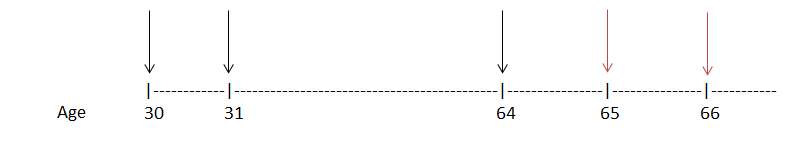
\includegraphics[width=0.7\textwidth]{images/timeDiagram}
\end{center}
\vspace{-5mm}
\caption{Cash flows for annual case}
\end{figure}

\subsection{Policyholder Ages}

Age is by far the most important factor to consider when setting premium levels. Intuitively, an older policyholder must pay significantly larger premiums. Reasons for this are twofold:

\begin{itemize}
\item The period until age 65 for an older policyholder is much shorter, so they make less payments than a younger policyholder.
\item Older policyholders receive the same annual benefit (\$50,000) as a younger policyholder, but receive these benefits sooner. Therefore, the benefit payments are less affected by the time value of money for older policyholders.
\end{itemize}

In fact, if one considers the total amount of premiums payed (over the life of the contact) by a policyholder for a product based on their age, the results are surprising. We found that a policyholder aged 60 could be paying 2.5 times more than a policyholder aged 30 for an equivalent benefits, if the present value of these payments is ignored. %\footnote{see Table \ref{table:markupTable}. (30) pays 5945.03*35 whereas (60) pays 105,475.90*5}

Because the older policyholders are paying larger premiums, their effect is greater on the portfolio. For this reason, considering the breakdown of policyholders by age becomes important. We were given that 20\% of policyholders fall between the ages of 30-40, 30\% between the ages of 40-50, and 50\% the ages of 50-60. Since we were not told how the number of

\begin{figure}[!ht]
\begin{center}
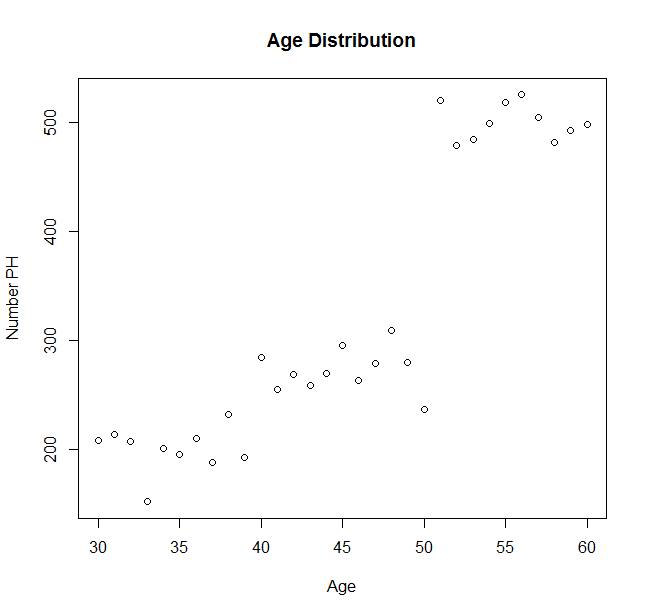
\includegraphics[width=0.6\textwidth]{images/ageDistribution}
\end{center}
\caption{Random policyholder numbers generated using a uniform distribution}
%\label{figure:agedistribution}
\end{figure}

Policyholders was distributed within each of these groups we decided to generate random numbers of policyholders as shown. The range of these random numbers was determined based on the proportionate size of the group when compared a total of 10,000 policyholders. %\footnote{alternative options include using the same number of PH at each age in a group, or an increasing function within a group}. Furthermore, in order to have each of the 31 possible ages represented in our calculations, we placed policyholders aged 40-50 (inclusive) in the second group of our age groups.

It is intuitive that group of policyholders who are older than age 50 should be the largest for this product. Younger aged people often lack the finances to pay premiums or may not be concerned about retirement at their current stage of life. As they approach retirement, however, they will likely start setting more money aside for this purpose.

\subsection{The Premium}

Our first approach at setting the premium, $\pi$, for this product was to equate the expected present value of future benefits and premiums. Under this approach, a new policyholder aged 30 would pay about \$5886.17 \footnote{This premium is calculated under a 10 year guarantee period}. In this particular case, the insurance company makes a profit on this policy only if the policyholder dies before 80.5. However, under our survival model, the probability of this policyholder surviving to age 80.5 is about 56\%. This means that if the insurance company was insuring only this policyholder, they could expect to lose money 56\% percent of the time! Clearly, since the insurance company has a responsibility to policyholders to pay out future benefits and does not want to go out of business, they must increase the number of policyholders or charge a larger premium.

\begin{figure}[!ht]
\begin{center}
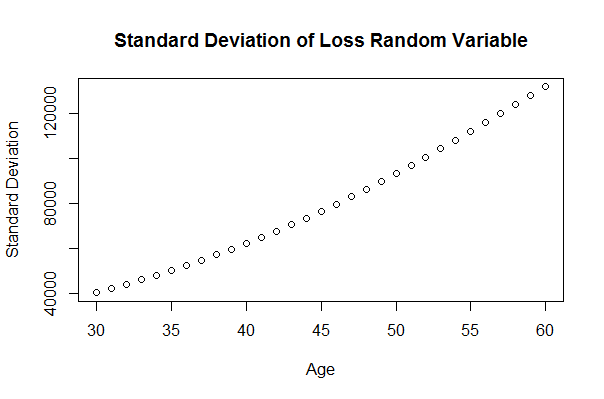
\includegraphics[width=0.6\textwidth]{images/stdevValues}
\end{center}
\vspace{-5mm}
\caption{Standard deviation of $L_{0}$ for contract with $n=10$ year guarantee period}
\label{figure:lossFunctionEPV}
\end{figure}

The challenge, as we will examine throughout the rest of the report, is how much larger of a premium to charge. When trying to markup this premium, at the forefront of our analysis was the balance between providing financial certainty to the insurer and charging affordable premiums.

\subsection{Concerns Regarding the Loss Function}

When we began aggregating the premiums, it became important to look at the standard deviation and expected value of the loss random variable for the entire portfolio. 

Before proceeding, we should point out that our options are limited when determining a premium markup to charge to the entire group. We cannot simply determine a break even point for the portfolio (as was did earlier for a single policyholder aged 30). Instead, we have chosen to assume that the losses in the portfolio are distributed normally, and standardize the aggregate loss for the portfolio by subtracting its expectation and dividing by its standard deviation.

Figure \ref{figure:lossFunctionEPV} shows the as age increases, the standard deviation of the loss random variable also increases. We earlier argued that most policyholders will be within the older age groups, so it makes sense that the standard deviation of our portfolio will be quite high ($\approx 9.0$ x $10^{6}$). 

If $L$ denotes the aggregate loss for the portfolio, and we use the premium determined by the equivalence principle, then $E(L)$ is 0 and $\sqrt{V(L)} \approx 9.0$ x $10^{6}$.   

It might seem strange at first that $V(L)$ is so large. However, earlier we argued that most policyholders will be within the older age groups. Since the contracts of older policyholders a high variance (see Figure \ref{figure:lossFunctionEPV}), it makes sense that the standard deviation of our portfolio will be quite high.

\begin{figure}[!ht]
\begin{center}
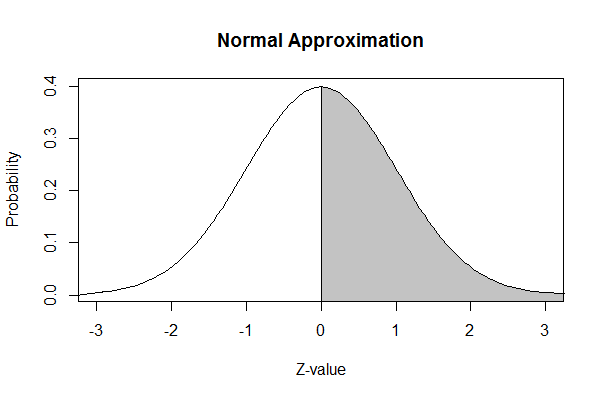
\includegraphics[width=0.5\textwidth]{images/normalPlot}
\end{center}
\caption{Probability of a loss (50\%) with no markup on premium}
\end{figure}

As shown above, under this method, the probability of a loss for the insured is 50\%. Clearly, this is unacceptable to the insurer.

If instead of charging $\pi_x$ to each policyholder, we were to charge 1.01$\pi_x$ (i.e.markup the price), we find that the standard deviation stays quite similar in value (slightly decreases). However, the expected loss on the entire portfolio drops dramatically (0 to $\approx 2.6$ x $10^{7}$). We then find that the probability of loss drops dramatically (below 1\%). In fact, to achieve a probability of loss that is 5\% we would only need to charge about 1.006$\pi_x$. 

\begin{figure}[!ht]
\begin{center}
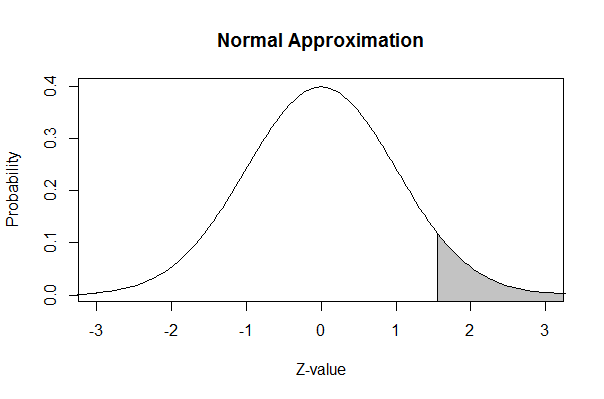
\includegraphics[width=0.6\textwidth]{images/normalPlot2}
\end{center}
\vspace{-5mm}
\caption{Probability of a loss (5\%) with a markup of 1.006 on premium}
\end{figure}

However, for reasons will examine next, we believe that a markup of 1.006 is too low.

\subsection{Premium Sensitivity to the Interest Rate}

Earlier, we stated that our analysis assumes an interest rate of 5\%. But what if our prediction is  wrong? What will happen to the premium if the interest rate changes?

From the insurer's perspective, it is most beneficial if the interest rate is high when they are collecting premiums (i.e. they can earn a lot of money on their reserves) and low when they are paying out premiums. However, these fluctuations in the interest rate are nearly impossible to predict.

\begin{table}[!ht]
\centering
\begin{tabular}{|c|ccc|ccc|}
\hline
& \multicolumn{3}{c}{$i = 5\% \to 4.5\%$} & \multicolumn{3}{|c|}{$i = 5\% \to 5.5\%$} \\
Age & $\Delta$ Benefit & $\Delta$ Premium & $\Delta \pi$ & $\Delta$ Benefit & $\Delta$ Premium & $\Delta \pi$ \\ [0.5ex]
\hline  
30 & 23.28\% & 6.24\% & 16.05\% & -18.72\% & -6.00\% & -16.05\% \\
40 & 17.53\% & 4.84\% & 12.12\% & -14.76\% & -4.70\% & -10.75\% \\
50 & 12.06\% & 3.14\%  & 8.64\% & -10.61\% & -3.08\%  & -7.86\% \\
\hline  
\end{tabular} 
\caption{Interest rate sensitivity}
\end{table}

If, instead of pricing premiums at 5\% interest, we did so at different rates (i.e. 4.5\% and 5.5\% as shown above), then the premium that we would charge would be different. Notice that the the benefit payments in particular are very sensitive to changes in the interest rate, since they only begin at age 65 (and thus are more effected by the time value of money). 

Another trend that should be pointed out is the premium charged to older ages is less effected by changes in the interest rate. Again, this can be explained by the shorter deferral period which older ages experience before their benefits begin. Therefore, the present values of their premium and benefit payments are less effected.

An important measure of the sensitivity of the price (in this case the premium) to changes in the interest rate is duration. The table below shows the effective durations associated with a change in the interest rate from 5\% in both directions. 

\begin{table}[!ht] 
\centering 
\begin{tabular}{c c c c c}
\hline
Age & 4.5\% & 5.0\% & 5.5\% & Duration\\ [0.5ex] 
\hline  
30 & 6830.51 & 5886.17 & 5071.49 & 0.299\\ 
40 & 16132.91 & 14236.25 & 12578.41 & 0.250\\ 
50 & 40586.57 & 36575.83 & 33048.39 & 0.206\\  
\hline  
\end{tabular} 
\caption{Effect of a change in the interest rate on premiums}  
\label{table:durationTable} 
\end{table} 

For instance, if the interest rate changes from 5.5\% to 4.5\%, then the approximate percentage change in premium would be 29.9\% for a 30 year old and 20.6\% for a 50 year old. Again, we see the trend that older ages are less effected by the interest rate. The durations are just another of this.

While it may be possible to account for the relationship between duration and age by charging a different markup to each age group, we decided not to do this \footnote{Justifying how much these markups should differ becomes difficult}. 

\subsection{Impact of the Interest Rate on the $Z$-Value}

As an insurance company, it is also important to discuss what happens to the probability of loss when the interest rate changes. 

Earlier, we mentioned that we did not believe a markup of 1.006 to be sufficient. To illustrate, let's say that we have priced our premium at 5\% interest rate. All seems to be going well, until suddenly, the interest rate falls to 4.5\%. If this happens, we are undercharging for premium. In an ideal world, we would be able to charge a larger premium to policyholders at this point, but unfortunately this is not an option.

\begin{table}[!ht] 
\centering 
\begin{tabular}{c c c c }
\hline
Interest Rate & Markup & $Z$-Value & Pr(Profit) \\ [0.5ex]
\hline  
0.045 & 1.01 & --12.84 & 0\% \\
0.05 & 1.01 & 4.48 & 99.9996 \% \\
0.055 & 1.01 & 23.36 & 100\% \\
\hline  
\end{tabular} 
\caption{Probability profit -- premium, benefit frequency $= 12$, guarantee period = 0}  
\label{table:grosspremiums} 
\end{table}

The table above illustrates the problem. If the interest rate were to drop and stay at 4.5\% for the entire life of these policies, then we would be guaranteed a loss. Alternatively, if the interest rate were to go up and stay at 5.5\% for the entire life of these policies, then we would be guaranteed a profit.

We notice (in Table \ref{table:grosspremiums2}) that if we were instead to charge a markup of 1.07, that we would fare much better. Even in a scenario in which the interest rate drops and stays at 4.5\%, we would still have some chance of making a profit (even though it is still slim). Indeed, at first glance, it may appear that we should use this a markup of 1.07 of even higher. However, some important considerations must be discussed which led us to instead choose the markup of 1.01.

\begin{table}[!ht] 
\centering 
\begin{tabular}{c c c c }
\hline
Interest Rate & Markup & Z-Value & Probability Profit \\ [0.5ex]
\hline  
0.045 & 1.07 & -0.60 & 27.44\% \\
0.05 & 1.07 & 18.07 & 100\% \\
0.055 & 1.07 & 38.37 & 100\% \\
\hline  
\end{tabular} 
\caption{Probability profit -- premium, benefit frequencies $=12$, guarantee period = 0}  
\label{table:grosspremiums2} 
\end{table} 

Firstly, we noticed that the expected variances of the loss random variable have already changed dramatically with a markup of 1.01. Larger markups continue to shift the expected value downwards until the insurance company is faced with no possible risk exposure at all. Doing so would guarantee the insurance company a very large profit. If the premiums charged are much larger than they need to be, this also raises ethical questions about the insurance company. 

\begin{figure}[!ht]
\centering
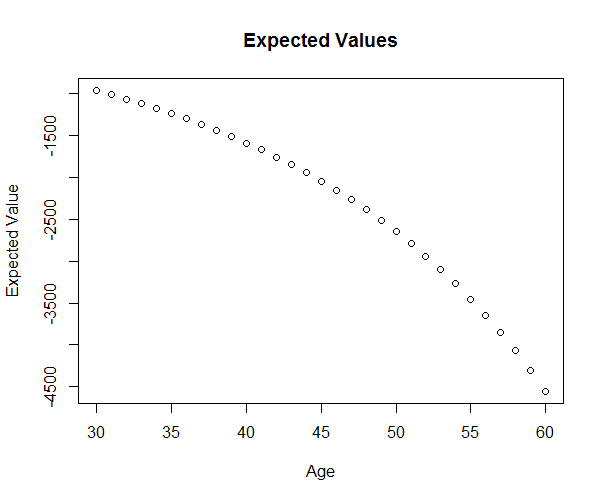
\includegraphics[width=0.5\textwidth]{images/expectedValuesMarkup}
\caption{Expected Values for Single Contract (Markup = 1.01)}
\label{figure:lossFunctionMarkup}
\end{figure}

\begin{figure}[!ht]
\begin{center}
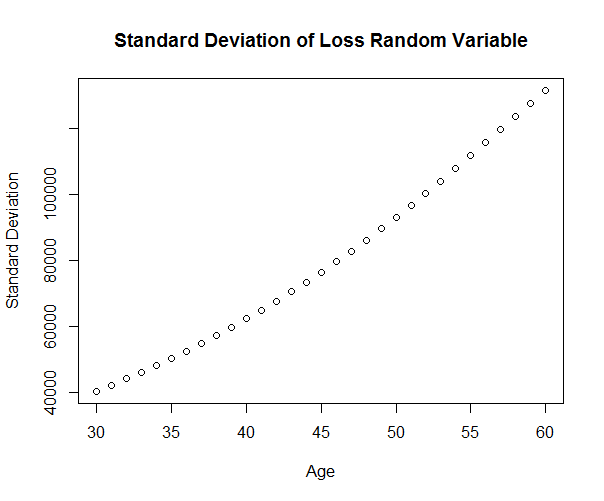
\includegraphics[width=0.5\textwidth]{images/stdevValuesMarkup}
\caption{Standard Deviation for Single Contract (Markup = 1.01)}
\end{center}
\end{figure}

Finally, while we realize it is possible for the insurance company to have a loss in the scenario described earlier (in which the interest rate is always lower than anticipated), we believe this is highly unlikely. After all, if the interest rate ends up fluctuating, it will likely do so in both directions (one of which is very profitable to us and one of which is not). 

\subsection{The Gross Premium and Closing Comments}

In Tables \ref{table:grosspremiums} and \ref{table:grosspremiums2}, we calculated probabilities with a guarantee period of 0 years, not with our usual of 10 years. We did so because a shorter guarantee period increases the variance of the loss function and is (in a sense) worse for the insurance company.

Table \ref{table:impactzvalue} further illustrates this point. It turns out that the options which policyholders choose directly effect the probability of a loss. In reality, it is hard to predict what policyholders will end up choosing, so as explained earlier, we assumed a ten year guarantee period on average as well as monthly frequencies.

\begin{table}[!ht] 
\centering 
\begin{tabular}{c c c c }
\hline
Option & Increase & Decrease & Significance \\ [0.5ex]
\hline  
premium Frequency & Decreases & Increases & Small\\
benefit Frequency & Increases & Decreases & Small \\
guarantee Period & Increases & Decreases & Large \\
\hline  
\end{tabular} 
\caption{Impact of changing parameters on the $z$-value}  
\label{table:impactzvalue} 
\end{table} 

That said, we feel confident that a markup of 1\% to the equivalence principle premium described earlier is appropriate. We believe this would allow the ABC insurance company to both charge an attractive price for the product and feel secure financially.

\newpage
\section{Appendices}

\subsection{Standard Select Survival Model}

For this retirement product, we have assumed that mortality follows the standard select survival model with $A=0.00022$, $B=2.5e-05$, $c=1.1$. In other words, we have assumed that $\mu_{x+s} = A + Bc^{x+s}$ and $\mu_{[x]+t}=0.9^{2-t}\mu_{x+t}$ for $0\le t \le 2$. Using the fact that $\hspace{0mm}_tp_x=e^{-\int_{0}^{t}u_{x+s}ds}$, we have that

\begin{align*}
\hspace{0mm}_tp_x = e^{-At + \frac{B}{ln(c)}c^x(c^t -1)}
\end{align*}

Similarly, we can derive a formula for $\hspace{0mm}_tp_{[x]}$ by integrating $e^{-\int_{0}^{t}u_{[x]+s}ds}$. Doing so, we get that 

\begin{align*}
\hspace{0mm}_tp_{[x]} = 
e^{0.9^{2-t}A\frac{(1 - 0.9^t)}{ln(0.9)} + Bc^x\frac{(c^t - 0.9^t)}{ln(0.9/c)}}
\end{align*}

which is valid for $0\le t \le 2$. Finally, since the select period is two years, we must also derive a formula for $\hspace{0mm}_tp_{[x]+1}$, namely

\begin{align*}
\hspace{0mm}_tp_{[x]+1} = 
e^{0.9^{1-t}A\frac{(1-0.9^t)}{ln(0.9)} + Bc^{x+1}\frac{(c^t - 0.9^t)}{ln(0.9/c)}}
\end{align*}

which is valid for $0\le t \le 1$.

\begin{figure}[!ht]
\centering
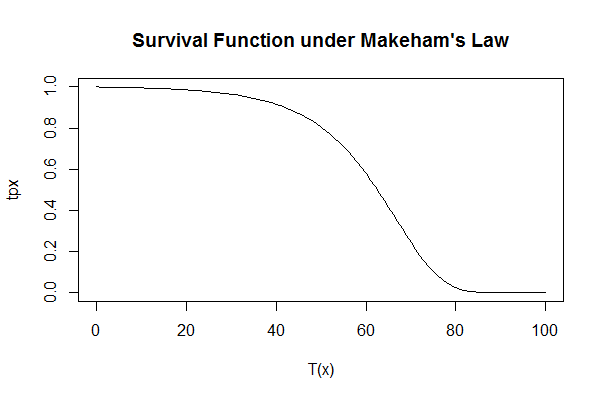
\includegraphics[scale=0.4]{images/makehamsplot}
\caption{Plots of $\hspace{0mm}_tp_x$ and $d_x$ under Makeham's Law}
\end{figure}

\begin{figure}[!ht]
\centering
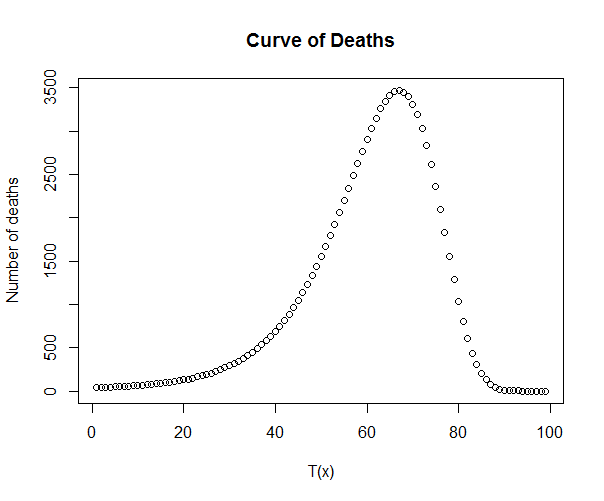
\includegraphics[scale=0.4]{images/makehamsdeaths}
\caption{Plots of $\hspace{0mm}_tp_x$ and $d_x$ under Makeham's Law}
\end{figure}

\subsection*{Benefit Outgo}

Let $Y$ denote the present value random variable for the benefit paid out. These payments will start at age 65 if (x) is still alive. Let $u=65-x$ denote this deferral period, where $x$ is the age of the insured when selected. The insured can choose a benefit frequency, $m_y$ and guarantee period, $n$

\begin{align*}
Y =
\begin{cases}
0 & k=0,\frac{1}{m_y},\dots{}, u-\frac{1}{m_y} \\
v^u\ddot{a}_{\lcroof{n}}^{(m_y)} & k=u,u+\frac{1}{m_y},\dots{},u+n-\frac{1}{m_y} \\
v^u\ddot{a}_{\lcroof{k+\frac{1}{m_y}-u}}^{(m_y)} & k = u+n,u+n+\frac{1}{m_y}, \dots{}
\end{cases}
\end{align*}

The expected value of Y equals to the expected value of a guarantee annuity issued to $(x+u)$ discounted back to time 0 for interest and survivorship

\begin{align*}
E(Y) &= u|\ddot{a}_{\overline{[x]:\lcroof{n}}}^{(m_y)} \\ 
&= uE_{[x]}\ddot{a}_{\overline{x+u:\lcroof{n}}}^{(m_y)}
\end{align*}

We can find the variance of Y by using an indicator random variable. %
\begin{align*}
I &=
\begin{cases}
0 & \text{if (x) dies before 65} \\
1 & \text{if (x) survives to 65}
\end{cases}
\end{align*}

\begin{align*}
E(Y|I=0) &= 0 \\
E(Y|I=1) &= \ddot{a}_{\overline{x+u:\lcroof{n}}}^{(m_y)} v^u  \\
V(Y|I=0) &=0 \\
V(Y|I=1) &= v^{2u}v^{2n}\hspace{0mm}_np_{x+u}(\hspace{0mm}_nq_{x+u}
(\ddot{a}_{x+u+n}^{(m_y)})^2 + \frac{\hspace{0mm}^2A_{x+u+n}^{(m_y)} - (A_{x+u+n}^{(m_y)})^2}{(d^{(m_y)})^2})
\end{align*}

Then we can apply the conditional variance formula, $V(Y)=E(V(Y|I)) + V(E(Y|I))$ 

\begin{align*}
E(V(Y|I)) &= \hspace{0mm}_up_{[x]}V(Y|I=1) \\
V(E(Y|I)) &= E(E(Y|I)^2) - E(E(Y|I))^2 \\
&= (v^{u}\ddot{a}_{\overline{x+u:\lcroof{n}}}^{(m_y)})^{2} 
\hspace{0mm}_up_{[x]} - (\hspace{0mm}_up_{[x]}v^{u}\ddot{a}_{\overline{x+u:\lcroof{n}}}^{(m_y)})^{2} \\
&= (v^{u}\ddot{a}_{\overline{x+u:\lcroof{n}}}^{(m_y)})^{2}\hspace{0mm}_up_{[x]} (1-\hspace{0mm}_up_{[x]})\\
&=  (v^{u}\ddot{a}_{\overline{x+u:\lcroof{n}}}^{(m_y)})^{2}\hspace{0mm}_up_{[x]}\hspace{1mm}_uq_{[x]}
\end{align*}

Combining these expressions together leads to the following formula for the variance

\begin{align*}
V(Y) &= \hspace{0mm}_up_{[x]}(
(v^{u}\ddot{a}_{\overline{x+u:\lcroof{n}}}^{(m_y)})^{2}\hspace{1mm}_uq_{[x]} +
(v^{u+n})^2\hspace{0mm}_np_{x+u}(\hspace{0mm}_nq_{x+u}
(\ddot{a}_{x+u+n}^{(m_y)})^2 + \frac{\hspace{0mm}^2A_{x+u+n}^{(m_y)} - (A_{x+u+n}^{(m_y)})^2}{(d^{(m_y)})^2})
)
\end{align*}

\subsection{Premium Income}

Let $Z$ denote the present value random variable for the premiums payed from (x) to 65. Let $m_z$ represent the premium frequency, and $u$ represent the deferral period as before.

\begin{align*}
Z &= 
\begin{cases}
\ddot{a}_{\lcroof{k+\frac{1}{m_z}}}^{(m_z)} & k=0,\frac{1}{m_z},\dots{}, u-\frac{1}{m_z} \\
\ddot{a}_{\lcroof{u}}^{(m_z)} & k=u,u+\frac{1}{m_z},\dots{},u+n-\frac{1}{m_z} \\
\ddot{a}_{\lcroof{u}}^{(m_z)} & k = u+n,u+n+\frac{1}{m_z}, \dots{}
\end{cases}
\end{align*}

Z is the present value random variable for a u-year temporary annuity payed $m^{thly}$ so its expected value and variance can be easily found using the following formulas

\begin{align*}
E(Z) &= \ddot{a}_{[x]:\lcroof{u}}^{(m_z)}\\
V(Z) &= \frac{\hspace{0mm}^2A_{x:\lcroof{u}}^{(m_z)} - (A_{x:\lcroof{u}}^{(m_z)})^{2}}{(d^{(m_z)})^2}
\end{align*}

\subsection{Covariance(Y,Z)}

Let $Y$ and $Z$ be defined as before. Then $YZ$ is a present value random variable defined as follows

\begin{align*}
YZ &= 
\begin{cases}
0 & k=0,\frac{1}{m},\dots{}, u-\frac{1}{m} \\
\ddot{a}_{\lcroof{u}}^{(m)}\ddot{a}_{\lcroof{n}}^{(m)} & k=u,u+\frac{1}{m},\dots{},u+n-\frac{1}{m} \\
\ddot{a}_{\lcroof{k+\frac{1}{m}}}^{(m)} & k = u+n,u+n+\frac{1}{m}, \dots{}
\end{cases}
\end{align*}

where $m$ represents the case in which $m_z$ = $m_y$ = $m$. If the two frequencies are not the same, the expression for $YZ$ becomes more complicated.

The covariance of $Y$ and $Z$ can be found using $Cov(Y,Z) = E(YZ) - E(Y)E(Z)$ where E(Y) and E(Z) are as derived above. The expression for $E(YZ)$ is 
%
\begin{align*}
E(YZ) = \hspace{0mm}_uE_{[x]}(\ddot{a}_{\lcroof{u}}^{(m_z)}\ddot{a}_{\lcroof{n}}^{(m_y)}
+v^n\hspace{0mm}_np_{x+u}\ddot{a}_{x+u+n}^{(m_y)}
)
\end{align*}

\subsection{The Loss Random Variable}

If $L_o(\pi) = Z-\pi{Y}$ then, $L_o(\pi)$ represents the loss random variable this retirement product. $L_o(\pi)$ can also be seen as prospective loss random variable at time 0. \\

If we use the equivalence principle to find a premium, we set $E(Lo(\pi)) = 0$ and solve for $\pi$. This premium will be
%
\begin{align*}
\pi &= \frac{E(Y)}{E(Z)} = \frac{u|\ddot{a}_{\overline{[x]:\lcroof{n}}}^{(m_y)}}{\ddot{a}_{[x]:\lcroof{u}}^{(m_z)}}
\end{align*}

And the variance becomes
\begin{align*}
V(Lo(\pi)) = \pi^2V(Z) + 50,000^2 V(Y) - 2(\pi)(50,000)Cov(Y,Z)
\end{align*}

\subsection{The Loss Function}

If the time of death is known, we can find the loss experienced by the insurer at different times based on a particular premium. Let $L(t,\pi)$ denote the loss function.

\begin{align*}
L_{0}(t,\pi) &= 
\begin{cases}
-\pi(\ddot{a}_{\lcroof{k+\frac{1}{m_z}}}^{(m_z)}) & k=0,\frac{1}{m_z},\dots{}, u-\frac{1}{m_z} \\
50,000v^u \ddot{a}_{\lcroof{n}}^{(m_y)} - \pi(\ddot{a}_{\lcroof{u}}^{(m_z)}) & k=u,u+\frac{1}{m_y},\dots{},u+n-\frac{1}{m_y} \\
50,000v^u \ddot{a}_{\lcroof{k+\frac{1}{m_y}-u}}^{(m_y)} - \pi(\ddot{a}_{\lcroof{u}}^{(m_z)}) & k = u+n,u+n+\frac{1}{m_y}, \dots{}
\end{cases}
\end{align*}

\begin{figure}[!ht]
\begin{center}
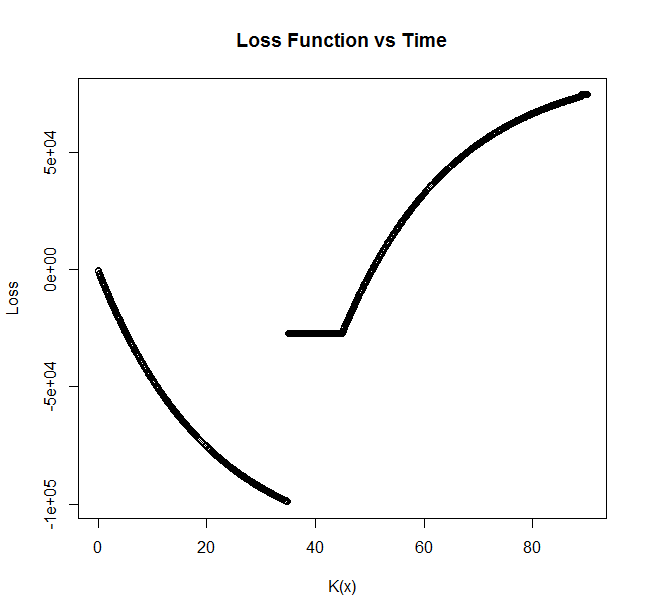
\includegraphics[width=0.5\textwidth]{images/lossFunction}
\end{center}
\vspace{-5mm}
\caption{Loss Function with $n=10$, $x=30$, $m_y=12$, $m_z=12$}
\label{figure:lossFunction}
\end{figure}

The probability density function can be found using the pdf of $K(x)$. $Pr(Lo(\pi))= C$ is $\hspace{0mm}_{k|}q_{[x]}$ for $k=0,1,\dots{},{w-x-1}$. If $m > 1 $, then at each $m^{thly}$ interval within a year, these probabilities are divided by $m$ (since UDD is assumed).

\begin{figure}[!ht]
\begin{center}
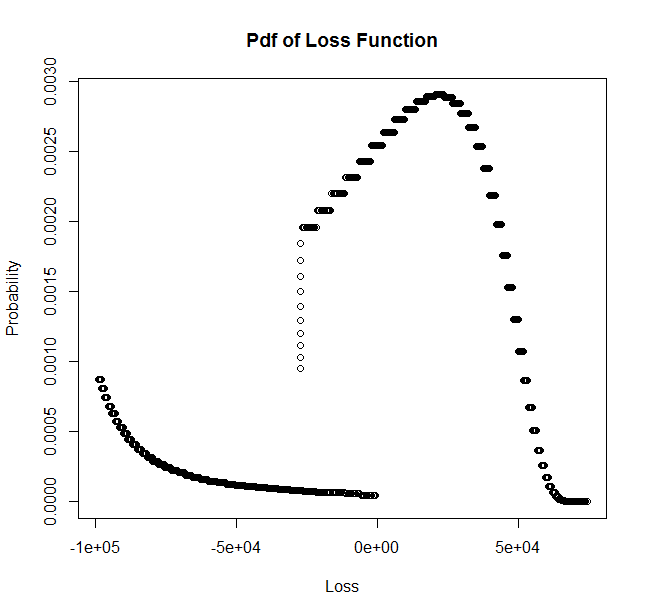
\includegraphics[width=0.5\textwidth]{images/pdfLossFunction}
\end{center}
\vspace{-5mm}
\caption{Pdf Loss Function with $n=10$, $x=30$, $m_y=12$, $m_z=12$}
\end{figure}

%\begin{figure}[!ht]
%\begin{center}
%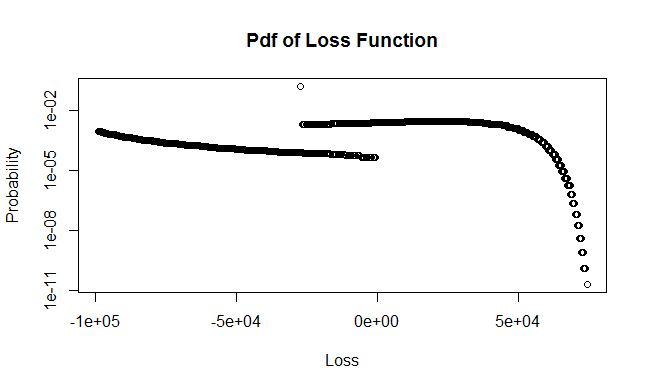
\includegraphics[width=0.4\textwidth]{images/addedpdf}
%\end{center}
%\caption{Pdf Loss Function with $n=10$, $x=30$, $m_y=12$, $m_z=12$}
%\label{figure:pdfLossFunction}
%\end{figure}

Note that there are two figures shown for the pdf plot. The one of the left does not combine the probabilities associated with a constant loss during the guarantee period. The one on the right does combine these probabilities. This plot also uses a logarithmic scale for the y-axis.

Finally, the cumulative distribution function can be found by sorting the losses (and corresponding probabilities) and then summing these probabilities. \footnote{see excel file for table of values corresponding to the loss function plots. note that the equivalence level premium to calculate loss values for these plots.}

\begin{figure}[!ht]
\begin{center}
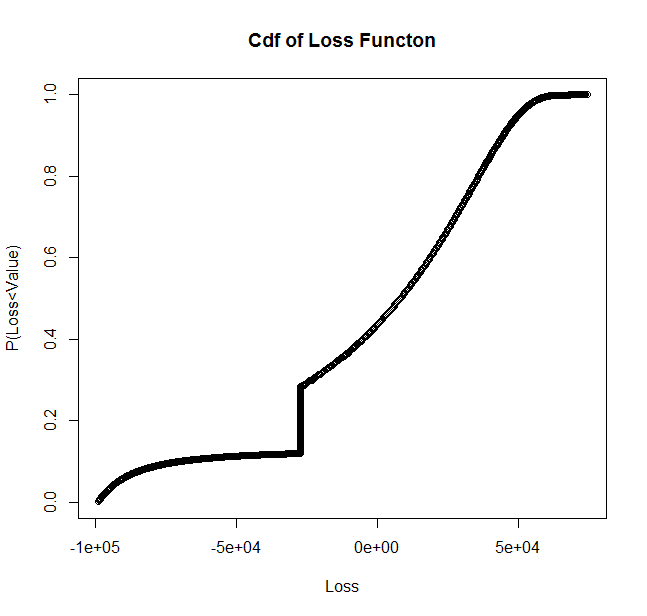
\includegraphics[width=0.5\textwidth]{images/cdfLossFunction}
\end{center}
\caption{Cdf of loss function with $n=10$, $x=30$, $m_y=12$, $m_z=12$}
\label{figure:cefLossFunction}
\end{figure}

\subsection{The Normal Approximation}

Let the premium charged to $(x)$ be denoted by $\pi_x$. Assuming that all policyholders aged $(x)$ have the same contract, then the expected loss at time 0 for these policyholders is $c_xE(Lo(\pi_x))$. The expected loss at time 0 for the whole portfolio can be calculated as $\sum_{x=30}^{60}c_xE(Lo(\pi_x))$. Similarly, the variance at time 0 for the whole portfolio (assuming independence) can be calculated as $\sum_{x=30}^{60}c_xV(Lo(\pi_x))$. If we then assume that losses are normally distributed for the portfolio, we can calculate the probability of a loss.

\begin{align*}
Pr(L>0) &\approx Pr(Z> \frac{0-E(L)}{\sqrt{V(L)}}) \\
&= 1 - Pr(Z< \frac{-E(L)}{V(L)}) 
\end{align*}

where $L$ represents the loss for the entire portfolio.

\subsection{Duration}

Because we are dealing with contingent cash flows which may change as a result of a change in the interest rate, we must use effective duration. The formula is

\begin{align*}
\mbox{Effective Duration} = \frac{PV_{i_{o-h}} - PV_{i_{o+h}}}{2h(PV_{i_o})}
\end{align*}

where h corresponds to a percentage change in the interest rate. This formula is used to calculate the duration corresponding to a change in the premium, with unit years. From earlier, we know that
$\pi= \frac{u|\ddot{a}_{\overline{[x]:\lcroof{n}}}^{(m_y)}}{\ddot{a}_{[x]:\lcroof{u}}^{(m_z)}}$. Using this formula, we can calculate the percentage change in the premium (based on a change in the interest rate) and find out how much of this change was caused by the benefit and premium streams. To calculate percentage change, use $\frac{P^* - P}{P}$ where $P^*$ is value at the new interest rate, and $P$ is the value at the original interest rate

\subsection{Detailed Pricing Tables}

The tables below represent our opinions on the premiums that should be charged for this product. We have omitted many of the intermediate values in order to shorten the length of the tables. For these tables, premium and benefit frequencies are both 12, the interest rate is 5\% and a markup of 1\% was used, for reasons discussed in the body of the report. 

% Mon Nov 09 18:51:59 2015
\begin{table}[ht]
\centering
\begin{tabular}{|r|rrr|rrr|}
  \hline
  & \multicolumn{3}{c}{No markup} & \multicolumn{3}{|c|}{1\% markup} \\ 
$x$ & $n=0$ & $n=10$ & $n=20$ & $n=0$ & $n=10$ & $n=20$ \\
  \hline
30 & 5,602.43 & 5,886.17 & 6,659.03 & 5,658.45 & 5,945.03 & 6,725.62 \\
31 & 5,956.39 & 6,258.06 & 7,079.75 & 6,015.96 & 6,320.64 & 7,150.55 \\
32 & 6,337.46 & 6,658.42 & 7,532.69 & 6,400.84 & 6,725.01 & 7,608.02 \\
33 & 6,748.33 & 7,090.10 & 8,021.05 & 6,815.82 & 7,161.00 & 8,101.26 \\
34 & 7,192.05 & 7,556.29 & 8,548.45 & 7,263.97 & 7,631.85 & 8,633.93 \\
35 & 7,672.07 & 8,060.62 & 9,119.00 & 7,748.79 & 8,141.23 & 9,210.19 \\
36 & 8,192.34 & 8,607.24 & 9,737.39 & 8,274.26 & 8,693.31 & 9,834.76 \\
37 & 8,757.36 & 9,200.88 & 10,408.97 & 8,844.94 & 9,292.89 & 10,513.06 \\
38 & 9,372.33 & 9,847.00 & 11,139.93 & 9,466.06 & 9,945.47 & 11,251.33 \\
39 & 10,043.25 & 10,551.89 & 11,937.37 & 10,143.68 & 10,657.41 & 12,056.75 \\
40 & 10,777.07 & 11,322.88 & 12,809.59 & 10,884.84 & 11,436.10 & 12,937.69 \\
41 & 11,581.93 & 12,168.50 & 13,766.25 & 11,697.75 & 12,290.19 & 13,903.91 \\
42 & 12,467.40 & 13,098.82 & 14,818.71 & 12,592.07 & 13,229.80 & 14,966.90 \\
43 & 13,444.79 & 14,125.71 & 15,980.44 & 13,579.24 & 14,266.97 & 16,140.25 \\
44 & 14,527.60 & 15,263.36 & 17,267.46 & 14,672.88 & 15,415.99 & 17,440.14 \\
45 & 15,732.03 & 16,528.78 & 18,699.04 & 15,889.35 & 16,694.07 & 18,886.03 \\
46 & 17,077.71 & 17,942.61 & 20,298.51 & 17,248.48 & 18,122.04 & 20,501.49 \\
47 & 18,588.67 & 19,530.10 & 22,094.43 & 18,774.55 & 19,725.40 & 22,315.38 \\
48 & 20,294.61 & 21,322.44 & 24,122.12 & 20,497.56 & 21,535.67 & 24,363.34 \\
49 & 22,232.71 & 23,358.69 & 26,425.73 & 22,455.04 & 23,592.28 & 26,689.99 \\
50 & 24,450.06 & 25,688.35 & 29,061.27 & 24,694.56 & 25,945.23 & 29,351.89 \\
51 & 27,007.29 & 28,375.08 & 32,100.78 & 27,277.36 & 28,658.83 & 32,421.79 \\
52 & 29,983.69 & 31,502.23 & 35,638.53 & 30,283.53 & 31,817.25 & 35,994.91 \\
53 & 33,485.09 & 35,180.95 & 39,800.27 & 33,819.94 & 35,532.76 & 40,198.28 \\
54 & 37,655.82 & 39,562.91 & 44,757.60 & 38,032.38 & 39,958.54 & 45,205.17 \\
55 & 42,698.08 & 44,860.54 & 50,750.81 & 43,125.06 & 45,309.14 & 51,258.32 \\
56 & 48,904.02 & 51,380.78 & 58,127.17 & 49,393.06 & 51,894.59 & 58,708.44 \\
57 & 56,712.01 & 59,584.20 & 67,407.72 & 57,279.13 & 60,180.05 & 68,081.80 \\
58 & 66,811.13 & 70,194.80 & 79,411.51 & 67,479.24 & 70,896.75 & 80,205.62 \\
59 & 80,350.18 & 84,419.54 & 95,503.98 & 81,153.68 & 85,263.73 & 96,459.02 \\
60 & 99,397.57 & 104,431.59 & 118,143.65 & 100,391.54 & 105,475.90 & 119,325.09 \\
   \hline
\end{tabular}
\caption{Detailed pricing table}
\end{table}

\end{document}
